\section{Geschäftsprozessmanagement}

\subsection{Grundlagen zu Geschäftsprozessen}
    \subsubsection*{Definition}
        Geschäftsprozesse sind die arbeitsteilige Ausführung von Aktivitäten in einer zeitlich-/sachlogischen Reihenfolge zur Erfüllung einer betrieblichen Aufgabe.
    \subsubsection*{Sichten}
        \begin{itemize}
            \item Steuerungssicht: Darstellung des Ablaufs eines Prozesses. Identifikation der Ereignisse (durch die ein Prozess ausgelöst wird bzw. die ein Prozess auslöst).
            \item Funktionssicht: Beschreibung und Zerlegung der Funktionen, die innerhalb eines Prozesses ausgeführt werden.
            \item Datensicht: Beschreibt Daten, die benötigt werden bzw. erzeugt werden.
            \item Organisationssicht: Beschreibt duch wen die Funktionen ausgeführt werden (z.B. Meschen oder Maschienen).
            \item Leistungssicht: Beschreibt die durch die Ausführung des Prozesses entstehenden Mehrwerte/Wertschöpfungen.
        \end{itemize}
    \subsubsection*{Arten}
        Wertschöpfende Kernprozesse, unterstützende Prozesse, Management Prozesse.
    \subsubsection*{Prozesstyp vs. Prozessinstanz}
        Typ ist die Vorlage, Instanz die konkrete Ausführung.

\subsection{Merkmale und Lebenszyklus des Geschäftsprozessmanagements}
    \subsubsection*{Ziele}
        Prozesse effektiver und effizienter gestalten.
    \subsubsection*{Rollen}
        \begin{itemize}
            \item Geschäftsführung: Verantwortlich für die grundsätzliche Gestaltung der Geschäftsprozesse.
            \item Prozessverantwortlicher: Verantwortlich für die Ausführung und Anpassung der Prozesse.
            \item Prozessteilnehmer: Führen Routineaufgaben innerhalb der Prozesse aus.
            \item Systemanalytiker: Erhebt, analysiert und verbessert Prozesse.
            \item Anwendungsentwickler: Verantwortlich für die softwaretechnische Umsetzung.
        \end{itemize}
    \subsubsection*{Lebenszyklus}
        \begin{figure}[h]
            \centering
            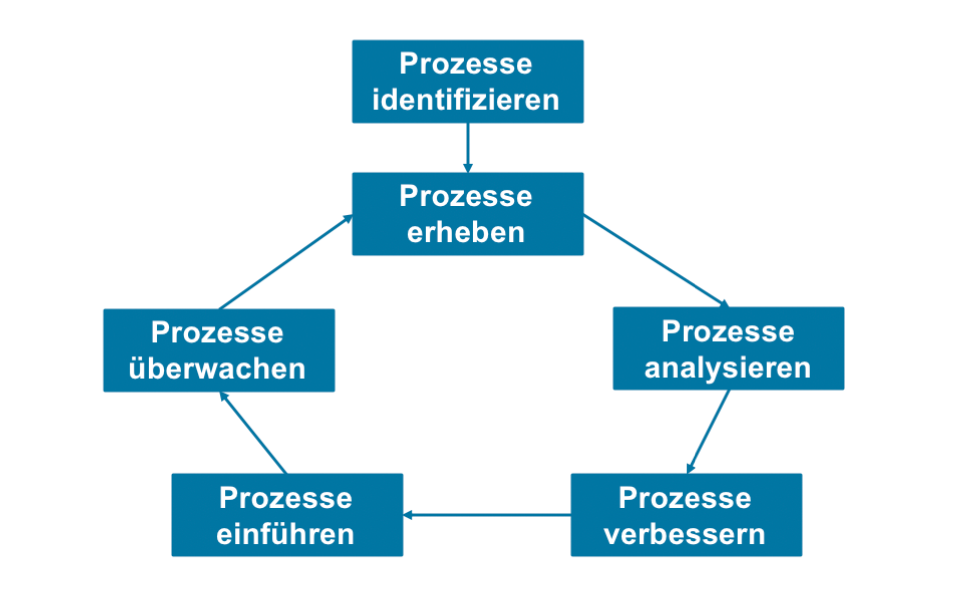
\includegraphics[width=\textwidth]{image/Lebenszyklus.png}
            \caption{Lebenszyklus Geschäftsprozessmanagements}
            \label{fig:Lebenszyklus}
        \end{figure}

\subsection{Identifikation von Geschäftsprozessen}
    \subsubsection*{Vorgehen}
        Erfassung der wichtigsten Prozesse, Darstellung als Prozesslandkarte oder Wertschöpfungskette, Bewertung und Auswahl der zu verbessernden Prozessen.
    \subsubsection*{Referenzmodelle}
        Dienen als Vorlagen zur Entwicklung spezifischer Prozesse. Bespiel: Handels-H-Modell (Abbildung \ref{fig:Handels-H-Modell}). Anerkannte Lösung für wiederkehrende Probleme.
        \begin{figure}[h]
            \centering
            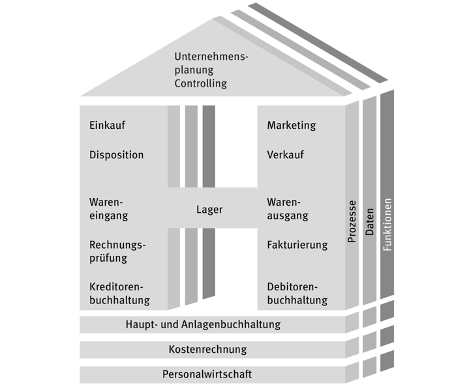
\includegraphics[width=\textwidth]{image/Handels-H-Modell.png}
            \caption{Handels H Modell}
            \label{fig:Handels-H-Modell}
        \end{figure}
    \subsubsection*{Techniken}
        Prozessmodellierung und -analyse zur Optimierung.

\subsection{Gestaltung von Geschäftsprozessen}
    \subsubsection{Prozesse erheben}
        \paragraph*{Ziel}
            Sammeln von Informationen über den aktuellen Ablauf eines Prozesses (IST-Modell).
        \paragraph*{Methoden}
            \begin{itemize}
                \item Dokumentensichtung: Nutzt vorhandene Dokumente, kann aber veraltet sein.
                \item Beobachtung: Direkte Erkennung des IST-Zustands, jedoch zeitaufwendig.
                \item Interviews: Detaillierte Informationen, aber zeitintensiv.
                \item Workshops: Kompakte und kollaborative Erhebung, jedoch zeitaufwendig für alle.
            \end{itemize}

    \subsubsection{Prozesse analysieren}
        \paragraph*{Ziel}
            Identifizieren von Schwachstellen und deren Ursachen.
        \paragraph*{Typische Schwachstellen}
            \begin{itemize}
                \item Lange Durchlaufzeiten
                \item Hohe Fehlerquote
                \item Hohe Kosten
                \item Geringe Flexibilität
            \end{itemize}
        \paragraph*{Methoden}
            \begin{itemize}
                \item Qualitative Analyse: Wertbeitragsanalyse, Ursache-Wirkungsdiagramme.
                \item Quantitative Analyse: Nutzung statistischer Daten zur Identifikation von Engpässen.
            \end{itemize}

    \subsubsection{Prozesse verbessern}
        \paragraph*{Ziel}
            Vorschläge zur Eliminierung von Schwachstellen und Erstellung eines SOLL-Prozesses.
        \paragraph*{Dimensionen der Verbesserung}
            Durchlaufzeit, Kosten, Qualität, Flexibilität. (Abbildung \ref{fig:Teufelsviereck})
            \begin{figure}[ht]
                \centering
                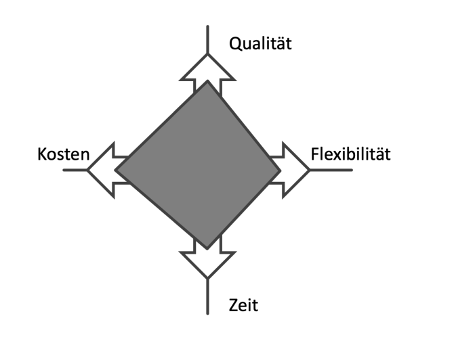
\includegraphics[width=\textwidth]{image/Teufelsviereck.png}
                \caption{Teufelsviereck}
                \label{fig:Teufelsviereck}
            \end{figure}
        \paragraph*{Methoden}
            \begin{itemize}
                \item Verbesserungsvorschläge in den genannten Dimensionen erarbeiten.
                \item Redesign-Heuristiken: Konkrete Maßnahmen zur Umgestaltung von Prozessen.
            \end{itemize}

\subsection{Ausführung von Geschäftsprozessen}
    \subsubsection*{Umsetzung}
        Prozesse in die Praxis umsetzen durch Implementierung und Anpassung von Anwendungssystemen.
    \subsubsection*{Beispiele}
        Implementierung neuer Systeme, Anpassung bestehender Systeme, Bereitstellung benötigter Geräte.

\subsection{Prozesse einführen}
    \subsubsection*{Definition}
        Organisatorische und technische Maßnahmen zur Bereitstellung der Infrastruktur.
    \subsubsection*{Maßnahmen}
        Mitarbeiterschulung, Schaffung neuer Stellen, Anpassung bestehender Stellen, Implementierung oder Anpassung von Anwendungssystemen.

\subsection{Prozesse überwachen}
    \subsubsection*{Prozessüberwachung}
        Überwachung anhand aufgezeichneter Daten.
    \subsubsection*{KPI (Key Performance Indicators)}
        Aggregation und Darstellung von Kennzahlen zur Überwachung und Identifikation von Optimierungspotentialen.